\documentclass[13pt,a4paper]{article}
\usepackage[spanish,es-nodecimaldot]{babel}	% Utilizar español
\usepackage[utf8]{inputenc}					% Caracteres UTF-8
\usepackage{graphicx}						% Imagenes
\usepackage[hidelinks]{hyperref}			% Poner enlaces sin marcarlos en rojo
\usepackage{fancyhdr}						% Modificar encabezados y pies de pagina
\usepackage{float}							% Insertar figuras
\usepackage[textwidth=390pt]{geometry}		% Anchura de la pagina
\usepackage[nottoc]{tocbibind}				% Referencias (no incluir num pagina indice en Indice)
\usepackage{enumitem}						% Permitir enumerate con distintos simbolos
\usepackage[T1]{fontenc}					% Usar textsc en sections
\usepackage{amsmath}						% Símbolos matemáticos
\usepackage[ruled,vlined]{algorithm2e}      % Pseudocódigo
\usepackage{xcolor}
\usepackage{listings}
% Para que acepten tíldes los listing
\lstset{     
     literate=%
         {á}{{\'a}}1
         {é}{{\'e}}1
         {í}{{\'i}}1
         {ó}{{\'o}}1
         {ú}{{\'u}}1
         {Á}{{\'A}}1
         {É}{{\'E}}1
         {Í}{{\'I}}1
         {Ó}{{\'O}}1 
         {Ú}{{\'U}}1
         {ñ}{{\~n}}1 
         {Ñ}{{\~N}}1 
         {¿}{{?``}}1 
         {¡}{{!``}}1
}
\usepackage{dsfont}

% ==============================================================================

\usepackage{caption, subcaption}
\usepackage[section]{placeins}
\makeatletter
\def\fps@figure{H}
\makeatother

\usepackage{booktabs}
\usepackage{longtable}
\usepackage{array}
\usepackage{multirow}
\usepackage{wrapfig}
\usepackage{colortbl}
\usepackage{pdflscape}
\usepackage{tabu}
\usepackage{threeparttable}
\usepackage{threeparttablex}
\usepackage[normalem]{ulem}
\usepackage{makecell}
\usepackage{xcolor}
\usepackage[bottom]{footmisc}

\makeatletter
\newcommand*{\centerfloat}{%
  \parindent \z@
  \leftskip \z@ \@plus 1fil \@minus \textwidth
  \rightskip\leftskip
  \parfillskip \z@skip}
\makeatother

% ==============================================================================
% ==============================================================================

% Comando para poner el nombre de la asignatura
\newcommand{\asignatura}{Big Data II}
\newcommand{\autor}{Ignacio Vellido Expósito}
\newcommand{\email}{ignaciove@correo.ugr.es}
\newcommand{\titulo}{Práctica}
\newcommand{\subtitulo}{Análisis de datos en Big Data}

% Configuracion de encabezados y pies de pagina
\pagestyle{fancy}
\lhead{\autor{}}
\rhead{\asignatura{}}
\lfoot{Máster Ciencia de Datos e Ingeniería de Computadores}
\cfoot{}
\rfoot{\thepage}
\renewcommand{\headrulewidth}{0.4pt}		% Linea cabeza de pagina
\renewcommand{\footrulewidth}{0.4pt}		% Linea pie de pagina

% ==============================================================================
% ==============================================================================

\begin{document}
    \pagenumbering{gobble}
    % ==============================================================================
% Pagina de titulo
\begin{titlepage}
    \begin{minipage}{\textwidth}
        \centering

        
\includegraphics[scale=0.5]{img/ugr.png}\\

        \textsc{\Large \asignatura{}\\[0.2cm]}
        \textsc{MÁSTER CIENCIA DE DATOS E INGENIERÍA DE COMPUTADORES}\\[1cm]

        \noindent\rule[-1ex]{\textwidth}{1pt}\\[1.5ex]
        \textsc{{\Huge \titulo\\[0.5ex]}}
        \textsc{{\Large \subtitulo\\}}
        \noindent\rule[-1ex]{\textwidth}{2pt}\\[2.5ex]

        \end{minipage}

        \vspace{0.3cm}

        \begin{minipage}{\textwidth}

        \centering

        \textbf{Autor}\\ {\autor{} \\ ignaciove@correo.ugr.es}\\[1.5ex]
        \vspace{0.4cm}

        
\includegraphics[scale=0.3]{img/etsiit.jpeg}
        
\includegraphics[scale=0.6]{img/master.png}

        \vspace{0.7cm}
        \textsc{Escuela Técnica Superior de Ingenierías Informática y de Telecomunicación}\\
        \vspace{1cm}
        \textsc{Curso 2020-2021}
    \end{minipage}
\end{titlepage}
% ==============================================================================
    
    \pagenumbering{arabic}
    \tableofcontents
    \thispagestyle{empty}				% No usar estilo en la pagina de indice

    \newpage

    % ==============================================================================

    \section{Introducción}

\subsection{Conjunto de datos}

% The data has been produced using Monte Carlo simulations. The first 8 features are kinematic properties measured by the particle detectors in the accelerator. The last ten features are functions of the first 8 features; these are high-level features derived by physicists to help discriminate between the two classes. There is an interest in using deep learning methods to obviate the need for physicists to manually develop such features. Benchmark results using Bayesian Decision Trees from a standard physics package and 5-layer neural networks and the dropout algorithm are presented in the original paper. The last 500,000 examples are used as a test set.n about your data set

Para esta práctica tenemos un subconjunto de SUSY Data Set (\url{https://archive.ics.uci.edu/ml/datasets/SUSY}), un problema de clasificación binaria donde existe un ratio de desbalanceo de 10-90. La tarea consiste en distinguir la señal que produce una partícula supersimétrica frente a una posible señal cde fondo que se puede captar.

El dataset cuenta con dos millones de datos (1.000.000 de entrenamiento, 1.000.000 de test) con 18 características numéricas reales, y las siguientes medidas estadísticas:

\begin{table}[H]
    \begin{tabular}{c|c|c|c|c||c|c|c|c|}
    \cline{2-9}
    \textbf{}                        & \multicolumn{4}{c||}{\textbf{Train}}                       & \multicolumn{4}{c|}{\textbf{Test}}                              \\ \hline
    \multicolumn{1}{|c|}{\textbf{Columna}} & \textbf{Max} & \textbf{Min} & \textbf{Mean} & \textbf{Variance} & \textbf{Max} & \textbf{Min} & \textbf{Mean} & \textbf{Variance} \\ \hline
    \multicolumn{1}{|c|}{\textbf{1}}          & 16.89  & 0.25   & 1.23    & 0.62        & 15.65  & 0.25   & 1.23    & 0.62              \\ \hline
    \multicolumn{1}{|c|}{\textbf{2}}          & 2.10   & -2.10  & -9.92e-4      & 0.79        & 2.10   & -2.10  & -4.19e-4      & 0.79              \\ \hline
    \multicolumn{1}{|c|}{\textbf{3}}          & 1.73   & -1.73  & -5.97e-4      & 1.00        & 1.73   & -1.73  & 0.00    & 1.00              \\ \hline
    \multicolumn{1}{|c|}{\textbf{4}}          & 17.73  & 0.42   & 1.11    & 0.53        & 18.18  & 0.42   & 1.11    & 0.53              \\ \hline
    \multicolumn{1}{|c|}{\textbf{5}}          & 2.05   & -2.05  & -3.46e-4      & 0.83        & 2.05   & -2.05  & 7.25e-5       & 0.83              \\ \hline
    \multicolumn{1}{|c|}{\textbf{6}}          & 1.73   & -1.73  & 6.71    & 1.00        & 1.73   & -1.73  & 0.00    & 1.00              \\ \hline
    \multicolumn{1}{|c|}{\textbf{7}}          & 21.00  & 9.42   & 1.34    & 1.14        & 21.00  & 7.19   & 1.33    & 1.14              \\ \hline
    \multicolumn{1}{|c|}{\textbf{8}}          & 1.74   & -1.72  & 0.00    & 1.00        & 1.74   & -1.72  & 0.00    & 1.00              \\ \hline
    \multicolumn{1}{|c|}{\textbf{9}}          & 23.38  & 7.69   & 1.22    & 1.16        & 22.56  & 9.23   & 1.22    & 1.16              \\ \hline
    \multicolumn{1}{|c|}{\textbf{10}}         & 16.93  & -15.33       & 0.06    & 1.73        & 17.69  & -13.10       & 0.06    & 1.74              \\ \hline
    \multicolumn{1}{|c|}{\textbf{11}}         & 14.93  & 0.26   & 1.14    & 0.43        & 15.73  & 0.26   & 1.14    & 0.43              \\ \hline
    \multicolumn{1}{|c|}{\textbf{12}}         & 14.36  & 0.00   & 1.21    & 0.45        & 14.99  & 0.00   & 1.21    & 0.45              \\ \hline
    \multicolumn{1}{|c|}{\textbf{13}}         & 5.81   & 0.00   & 1.04    & 0.23        & 6.03   & 0.00   & 1.04    & 0.23              \\ \hline
    \multicolumn{1}{|c|}{\textbf{14}}         & 20.68  & 0.00   & 1.05    & 0.92        & 14.57  & 0.00   & 1.06    & 0.92              \\ \hline
    \multicolumn{1}{|c|}{\textbf{15}}         & 14.89  & 0.05   & 1.14    & 0.42        & 15.78  & 0.05   & 1.14    & 0.42              \\ \hline
    \multicolumn{1}{|c|}{\textbf{16}}         & 15.61  & 0.00   & 1.15    & 0.47        & 11.33  & 0.00   & 1.15    & 0.47              \\ \hline
    \multicolumn{1}{|c|}{\textbf{17}}         & 1.59   & 8.22   & 1.01    & 0.18        & 1.59   & 2.57   & 1.01    & 0.18              \\ \hline
    \multicolumn{1}{|c|}{\textbf{18}}         & 1.0    & 3.52   & 0.27    & 0.04        & 1.0    & 5.89   & 0.27    & 0.04              \\ \hline
    \end{tabular}
    \caption{Medidas estadísticas del conjunto de datos.}
    \label{statistics}
\end{table}

En base a la descripción del dataset en la página de la UCI, las primeras 8 características reflejan propiedades de las partículas medidas en un acelerador, y las 10 siguientes indican el resultado de diferentes funciones a partir de estas variables. Estas variables derivadas no aportan información nueva pero indica que puede resultar de ayuda en la clasificación de la fila.

\vspace{\baselineskip}

Tal y como vemos en la Tabla \ref{statistics}, las columnas del conjunto de datos se distribuyen en rangos diferentes, aunque de manera similar entre entrenamiento y test. Por ello, normalizaremos los datos antes de pasarlos por los algoritmos, haciendo uso del conjunto de funciones de KeelParser.

\newpage

\subsection{Técnicas aplicadas}

Las diferentes técnicas aplicadas en esta práctica son:
\begin{itemize}
    \item \textbf{De aprendizaje}: \begin{itemize}
        \item Árboles de decisión (MLlib.tree.DecisionTree).
        \item Random Forest (MLlib.tree.RandomForest).
        \item PCARD (MLlib.tree.PCARD).
        \item kNN-IS (MLlib.classification.kNN\_IS).
    \end{itemize}
    \item \textbf{De preprocesamiento}: \begin{itemize}
        \item \textbf{Selección de características}: \begin{itemize}
            \item Principal Component Analysis.
        \end{itemize}
        \item \textbf{Ajuste de desbalanceo}: \begin{itemize}
            \item Random Oversampling.
            \item Random Undersampling.
        \end{itemize}
        \item \textbf{Filtrado de ruido}: \begin{itemize}
            \item Homogeneous Ensemble (HME).
            \item NCNEdit.
        \end{itemize}
        \item \textbf{Selección de instancias}: \begin{itemize}
            \item FCNN.
            \item SSMA-SFLSDE.
        \end{itemize}
    \end{itemize}
\end{itemize}

La metodología seguida durante la práctica consistió comparar el mayor número de combinaciones posibles, no por ello reflexionando sobre la coherencia en el uso conjunto de algunas de ellas. En este caso, puesto que en el algoritmo PCARD aplica a los datos de entrada PCA, no se ha aplicado ninguna técnica de reducción de características en sus experimentos.

Para hacer esta exploración de flujos los algoritmos fueron entrenados con unos parámetros por defecto. Finalmente, a partir de los mejores resultados obtenidos para cada método, se realizó una optimización de los hiperparámetros para alcanzar el mayor valor de TPR x TNR posible.

\vspace{\baselineskip}

El flujo de técnicas de preprocesamiento de acorde a su uso es el siguiente:
\begin{enumerate}
    \item Selección de características
    \item Under|Over-sampling
    \item Filtrado de ruido
    \item Selección de instancias
\end{enumerate}

\vspace{\baselineskip}

La justificación es la siguiente: En base al conjunto de datos de entrenamiento con el que contamos, pretendemos reducir la dimensionalidad sin perder excesiva información. Puesto que el dataset cuenta con un ratio de desbalanceo del 90\%, RO y RU ajustan los datos para evitar un sesgo en las técnicas de clasificación. El uso de estas técnicas puede generar ruido adicional además del propio ruido inherente que debemos suponer que existe en nuestros datos, por lo que aplicamos técnicas de filtrado para eliminarlo. Finalmente, para agilizar el proceso de clasificación, seleccionamos el conjunto de instancias con mayor varianza del conjunto.

\vspace{\baselineskip}

A continuación se indican los parámetros utilizados en cada una de las técnicas:

\begin{itemize}
    \item \textbf{De aprendizaje}: \begin{itemize}
        \item \textbf{Árboles de decisión}: Se entrenan árboles con medida GINI, máxima profundidad de 5 y número de particiones a 32.
        \item \textbf{Random Forest}: De igual manera, los árboles se entrenan con medida GINI, máxima profundidad de 5 y número de particiones a 32. Se limita el número máximo de árboles entre 100 y 150.
        \item \textbf{PCARD}: El número de cortes se fija a 5, y el número de árboles entre 10 y 15.
        \item \textbf{kNN-IS}: Utilizando distancia euclídea, movemos el valor de k entre 5 y 7 y el de particiones a 10.
    \end{itemize}
    \item \textbf{De preprocesamiento}: \begin{itemize}
        \item \textbf{Selección de características}: \begin{itemize}
            \item \textbf{Principal Component Analysis}: Reducción al 50\% (9 características).
        \end{itemize}
        \item \textbf{Ajuste de desbalanceo}: \begin{itemize}
            \item \textbf{Random Oversampling}: Incremento del 50\%.
            \item \textbf{Random Undersampling}: Decremento hasta alcanzar igualdad en el número de instancias por clase.
        \end{itemize}
        \item \textbf{Filtrado de ruido}: \begin{itemize}
            \item \textbf{Homogeneous Ensemble (HME)}: Número de árboles fijado a 100, con máxima profundidad de 10 y 4 particiones.
            \item \textbf{NCNEdit}: Se consideran los 3 vecinos más cercanos.
        \end{itemize}
        \item \textbf{Selección de instancias}: \begin{itemize}
            \item \textbf{FCNN}: Se consideran los 3 vecinos más cercanos.
            \item \textbf{SSMA-SFLSDE}.
        \end{itemize}
    \end{itemize}
\end{itemize}
 \newpage
    \section{Análisis de resultados}

En esta sección se pretenden analizar aquellos resultados más relevantes. Algunos argumentos también se sustentan sobre las tablas completas de experimentos (con información adicional sobre ellos) que se encuentran en la sección \textit{Tablas de resultados}.

% Hay que describir detalladamente todo el proceso algorítmico utilizado, mostrando los resultados de cada uno de los algoritmos utilizados para entrenamiento y test, analizando el comportamiento, y mostrando los flujos/combinaciones de algoritmos de preprocesamiento

\vspace{\baselineskip}

\begin{table}[H]
    \centering
    \begin{tabular}{|l|c|c|c|c|r|}
    \hline
    \textbf{Algoritmo} & \textbf{\shortstack{Selección de \\ características}} & \textbf{\shortstack{Under/Over \\ sampling}} & \multicolumn{1}{l|}{\textbf{\shortstack{Filtrado \\ de ruido}}} & \multicolumn{1}{l|}{\textbf{\shortstack{Selección de \\ instancias}}} & \textbf{\shortstack{TPR \\ x \\ TNR}} \\ \hline
    Decision Tree      & No & RUS  & HME & FCNN  & 0.606 \\ \hline
    Random Forest      & No & RUS  & HME & FCNN  & 0.607 \\ \hline
    PCARD              & -  & RUS  & No  & No    & 0.598 \\ \hline
    kNN-IS             & No & RUS  & HME & No    & 0.526 \\ \hline
    \end{tabular}
    \caption{Flujos de preprocesamiento para los mejores resultados de cada algoritmo tras la optimización de parámetros.}
    \label{final}
\end{table}

Todos los valores de TPR x TNR mostrados son calculados sobre el conjunto de test.

% \subsection{Conclusiones generales}
% Objetivamente la calidad de los resultados es bastante superior a la baseline (cuánto ?), pero no por ello un tanto bajas. La práctica se ha enfocado en evaluar las diferentes combinaciones de técnicas (independientemente del resultado obtenido ?REALLY?). Una posible forma de mejorar sería un ajuste mayor de los hiperparámetros ???

\subsection{Sobre las técnicas de aprendizaje}

En términos de los algoritmos de clasificación, tal y como se muestra en la tabla \ref{final}, obtenemos prácticamente la misma calidad con cualquiera de ellos (con variación de milésimas), siendo ligeramente superior Random Forest (RF) y Árboles de Decisión (DT). Para ambas técnicas el flujo de preprocesamiento coincide, reduciendo enormemente el tamaño del conjunto de datos a un 10\% del tamaño original.

Mediante las tablas \ref{dt} y \ref{rf} vemos que independientemente del preprocesamiento los resultados son muy similares para las dos técnicas, probablemente debido al estar un algoritmo formado como ensamblado del otro. A pesar de esto, vemos que en media RF es más robusto con RUS mientras que DT funciona mejor con ROS.

\vspace{\baselineskip}

Sobre PCARD, aunque la calidad máxima se alcanza con las mínimas técnicas de preprocesamiento (ajustar el desbalanceo es imprescindible en este problema, y los resultados lo demuestran) no llega a ser significativamente inferior que el resto. 

Además, a partir de la tabla \ref{pcard} notamos que las técnicas NCNEdit y FCNN empeoran los resultados frente a no usar ninguna. Creemos que el motivo reside en que al aplicar PCARD PCA antes de entrenar los árboles, se pierde demasiada información al haber reducido el conjunto de datos con los algoritmos de filtrado de ruido y reducción de instancias.
% Qué pasa con HME ??

\vspace{\baselineskip}

Respecto a kNN, notamos peor calidad independientemente de la técnica y parámetros con los que se ha probado. Sin hacer un análisis de la distribución de los datos el razonamiento no está claro, pues al ser un algoritmo basado en distancias si existen alto entremezclado entre los elementos de la clase es de esperar con los pocos valores de k que se ha probado sea insuficiente.

% Es incluso posible que el filtrado de ruido 
% Fijándonos en que obtiene una precisión de 0.887 cuando no se aplica ningún preprocesamiento, deducimos que existen una buena cantidad de puntos entremezclados en el espacio - MEJOR NO PONER

\newpage

\subsection{Sobre las técnicas de selección de características}

Como se dijo anteriormente, hemos aplicado PCA únicamente a los algoritmos donde tiene sentido, pero podemos ver a partir de la tabla \ref{avg} y la de cada algoritmo que los resultados empeoran tras su uso.

\vspace{\baselineskip}

Hacemos notar que PCARD se comporta mejor que los árboles de decisión con PCA, a pesar de acabar teniendo un flujo similar. El razonamiento lo achacamos a la discretización aleatoria (RD) de PCARD, que elige un tamaño de intervalos mejor que el de 32 con el que se han entrenado los árboles.

\vspace{\baselineskip}

A pesar de todo, podríamos considerar si la reducción de dimensionalidad conseguida es aceptable a costa de esa cantidad de empeoramiento. En este problema, pasando de una media de 0,593 a 0,584, que corresponde a una clasificación errónea de $593.000 - 584.000 = 9.000$ instancias más, dada la semántica del problema no parece una pérdida substancial. Si por otro caso tratáramos con un problema médico habría que considerar independientemente el TPR y el TNR antes de aceptar esta conclusión.

\subsection{Sobre las técnicas de balanceo de datos}

No solo RUS ayuda a acelerar la tarea de aprendizaje, también nos da los mejores resultados. Aún así, en media vemos que se comporta peor que ROS, debido probablemente a que su combinación con técnicas de selección de instancias reduce en algunos casos de manera excesiva el conjunto de datos.

\subsection{Sobre las técnicas de reducción de ruido}

Los resultados dan a entender de que el dataset no es de por sí bastante ruidoso, y el posible ruido introducido por las otras técnicas no resulta influyente. No por ello dejamos de apreciar que HME ayuda en la obtención de los mejores valores de TPR x TNR y funciona mejor en este conjunto de datos que NCNEdit.

\subsection{Sobre las técnicas de reducción de instancias}

Vemos que el uso de FCNN apenas altera los resultados, pero no por ello deja de ser útil, pues aplica una reducción en torno al 50\% del conjunto de datos. En una situación de big data como la que nos encontramos esto es totalmente deseable, ya que reducimos tiempo de cómputo y carga en el sistema.

\vspace{\baselineskip}

Finalmente, indicamos que aunque la técnica SSMA sobrepasa el límite de 4GB de memoria impuesto en la práctica, en base a las dos ejecuciones con las que contamos (de los primeros días cuando el límite estaba en 46GB) vemos que la reducción en el número de instancias es extremadamente grande, llegando a obtener subconjuntos de 12.000 y 20.000 instancias.
A pesar de ello en este caso los resultados sí son bastante inferiores respecto a FCNN o no aplicar nada, por lo que concluímos que su uso no es positivo en este conjunto de datos.

\begin{table}
    \centering
    \begin{tabular}{cc|c|c|c|}
    \cline{3-5}
    \multicolumn{1}{l}{\textbf{}} & \textbf{} & \multicolumn{1}{c|}{\textbf{Average}} & \multicolumn{1}{c|}{\textbf{STD}} & \textbf{Max} \\ \hline
    \multicolumn{1}{|c|}{\multirow{3}{*}{Filtrado de ruido}}       & No        & 0.282  & 0.234
    & 0.565    \\ \cline{2-5} 
    \multicolumn{1}{|c|}{}  & HME       & 0.339   & 0.226    & 0.575        \\ \cline{2-5} 
    \multicolumn{1}{|c|}{}  & NCNEdit   & 0.273   & 0.249    & 0.564        \\ \hline
    \multicolumn{1}{|c|}{\multirow{2}{*}{Selección de instancias}} & No        & 0.321  & 0.244    & 0.575        \\ \cline{2-5} 
    \multicolumn{1}{|c|}{}  & FCNN      & 0.277   & 0.219    & 0.574        \\ \hline
    \multicolumn{1}{|c|}{\multirow{2}{*}{Selección de características}} & No        & 0.328  & 0.214    & 0.593        \\ \cline{2-5} 
    \multicolumn{1}{|c|}{}  & PCA      & 0.252    & 0.225    & 0.584        \\ \hline
    \multicolumn{1}{|c|}{\multirow{3}{*}{Balanceo de datos}}       & No        & 0.070  & 0.092    & 0.208        \\ \cline{2-5} 
    \multicolumn{1}{|c|}{}  & ROS       & 0.415   & 0.229    & 0.521        \\ \cline{2-5} 
    \multicolumn{1}{|c|}{}  & RUS       & 0.373   & 0.210    & 0.575        \\ \hline
    \end{tabular}
    \caption{Media de resultados de las diferentes técnicas de preprocesamiento.}
    \label{avg}
\end{table}

\begin{table}
    \centering
    \begin{tabular}{cc|c|c|c|}
    \cline{3-5}
    \multicolumn{1}{l}{\textbf{}} & \textbf{} & \multicolumn{1}{c|}{\textbf{Average}} & \multicolumn{1}{c|}{\textbf{STD}} & \textbf{Max} \\ \hline
    \multicolumn{1}{|c|}{\multirow{3}{*}{Filtrado de ruido}}       & No        & 0.288 & 0.253
    & 0.589    \\ \cline{2-5} 
    \multicolumn{1}{|c|}{}  & HME       & 0.339 &  0.231
    & 0.593        \\ \cline{2-5} 
    \multicolumn{1}{|c|}{}  & NCNEdit   & 0.292 &  0.255
    & 0.584        \\ \hline
    \multicolumn{1}{|c|}{\multirow{2}{*}{Selección de instancias}} & No        & 0.333  & 0.256
    & 0.597        \\ \cline{2-5} 
    \multicolumn{1}{|c|}{}  & FCNN      & 0.289 &  0.231
    & 0.593        \\ \hline
    \multicolumn{1}{|c|}{\multirow{2}{*}{Selección de características}} & No        & 0.341  &  0.241
    & 0.593        \\ \cline{2-5} 
    \multicolumn{1}{|c|}{}  & PCA      & 0.272  & 0.242
    & 0.584        \\ \hline
    \multicolumn{1}{|c|}{\multirow{3}{*}{Balanceo de datos}}       & No        & 0.066  &  0.070
    & 0.215        \\ \cline{2-5} 
    \multicolumn{1}{|c|}{}  & ROS       & 0.426 &  0.136
    & 0.542        \\ \cline{2-5} 
    \multicolumn{1}{|c|}{}  & RUS       & 0.284 &  0.273
    & 0.593        \\ \hline
    \end{tabular}
    \caption{Efectos de las diferentes técnicas de preprocesamiento para árboles de decisión.}
    \label{dt}
\end{table}

\begin{table}
    \centering
    \begin{tabular}{cc|c|c|c|}
    \cline{3-5}
    \multicolumn{1}{l}{\textbf{}} & \textbf{} & \multicolumn{1}{c|}{\textbf{Average}} & \multicolumn{1}{c|}{\textbf{STD}} & \textbf{Max} \\ \hline
    \multicolumn{1}{|c|}{\multirow{3}{*}{Filtrado de ruido}}       & No        & 0.239  & 0.250
    & 0.583    \\ \cline{2-5} 
    \multicolumn{1}{|c|}{}  & HME       & 0.294  & 0.238
    & 0.587        \\ \cline{2-5} 
    \multicolumn{1}{|c|}{}  & NCNEdit   & 0.222  & 0.252
    & 0.585        \\ \hline
    \multicolumn{1}{|c|}{\multirow{2}{*}{Selección de instancias}} & No        & 0.278   & 0.257
    & 0.585        \\ \cline{2-5} 
    \multicolumn{1}{|c|}{}  & FCNN      & 0.224  & 0.229
    & 0.587        \\ \hline
    \multicolumn{1}{|c|}{\multirow{2}{*}{Selección de características}} & No        & 0.316  &  0.258
    & 0.587        \\ \cline{2-5} 
    \multicolumn{1}{|c|}{}  & PCA      & 0.187   & 0.211
    & 0.511        \\ \hline
    \multicolumn{1}{|c|}{\multirow{3}{*}{Balanceo de datos}}       & No        & 0.039  & 0.184
    & 0.196        \\ \cline{2-5} 
    \multicolumn{1}{|c|}{}  & ROS       & 0.353  & 0.273
    & 0.532        \\ \cline{2-5} 
    \multicolumn{1}{|c|}{}  & RUS       & 0.362  & 0.179
    & 0.587        \\ \hline
    \end{tabular}
    \caption{Efectos de las diferentes técnicas de preprocesamiento para Random Forest.}
    \label{rf}
\end{table}

\begin{table}
    \centering
    \begin{tabular}{cc|c|c|c|}
    \cline{3-5}
    \multicolumn{1}{l}{\textbf{}} & \textbf{} & \multicolumn{1}{c|}{\textbf{Average}} & \multicolumn{1}{c|}{\textbf{STD}} & \textbf{Max} \\ \hline
    \multicolumn{1}{|c|}{\multirow{3}{*}{Filtrado de ruido}}       & No        & 0.309   & 0.273
    & 0.597        \\ \cline{2-5} 
    \multicolumn{1}{|c|}{}  & HME       & 0.369   &  0.241
    & 0.595        \\ \cline{2-5} 
    \multicolumn{1}{|c|}{}  & NCNEdit   & 0.286   &  0.290
    & 0.593        \\ \hline
    \multicolumn{1}{|c|}{\multirow{2}{*}{Selección de instancias}} & No        & 0.362   & 0.268
    & 0.597        \\ \cline{2-5} 
    \multicolumn{1}{|c|}{}  & FCNN      & 0.281   & 0.252
    & 0.595        \\ \hline
    \multicolumn{1}{|c|}{\multirow{3}{*}{Balanceo de datos}}       & No        & 0.072   & 0.076
    & 0.186        \\ \cline{2-5} 
    \multicolumn{1}{|c|}{}  & ROS       & 0.496   & 0.325
    & 0.542        \\ \cline{2-5} 
    \multicolumn{1}{|c|}{}  & RUS       & 0.397   & 0.220
    & 0.597        \\ \hline
    \end{tabular}
    \caption{Efectos de las diferentes técnicas de preprocesamiento para PCARD.}
    \label{pcard}
\end{table}

\begin{table}
    \centering
    \begin{tabular}{cc|c|c|c|}
    \cline{3-5}
    \multicolumn{1}{l}{\textbf{}} & \textbf{} & \multicolumn{1}{c|}{\textbf{Average}} & \multicolumn{1}{c|}{\textbf{STD}} & \textbf{Max} \\ \hline
    \multicolumn{1}{|c|}{\multirow{3}{*}{Filtrado de ruido}}       & No        & 0.292  & 0.159
    & 0.491    \\ \cline{2-5} 
    \multicolumn{1}{|c|}{}  & HME       & 0.354   & 0.193
    & 0.525        \\ \cline{2-5} 
    \multicolumn{1}{|c|}{}  & NCNEdit   & 0.294  & 0.200
    & 0.492        \\ \hline
    \multicolumn{1}{|c|}{\multirow{2}{*}{Selección de instancias}} & No        & 0.313    &  0.195
    & 0.525        \\ \cline{2-5} 
    \multicolumn{1}{|c|}{}  & FCNN      & 0.313   &  0.165
    & 0.521        \\ \hline
    \multicolumn{1}{|c|}{\multirow{2}{*}{Selección de características}} & No        & 0.328    & 0.177
    & 0.525        \\ \cline{2-5} 
    \multicolumn{1}{|c|}{}  & PCA      & 0.299   & 0.188
    & 0.516        \\ \hline
    \multicolumn{1}{|c|}{\multirow{3}{*}{Balanceo de datos}}       & No        & 0.103     &  0.038
    & 0.235        \\ \cline{2-5} 
    \multicolumn{1}{|c|}{}  & ROS       & 0.386  & 0.180
    & 0.432        \\ \cline{2-5} 
    \multicolumn{1}{|c|}{}  & RUS       & 0.448  & 0.167
    & 0.525        \\ \hline
    \end{tabular}
    \caption{Efectos de las diferentes técnicas de preprocesamiento para kNN.}
    \label{knn}
\end{table} \newpage
    \section{Resultados globales}

Orden usado en las técnicas:
Under/Oversampling > NoiseFiltering > Instance Selection

\begin{figure}[ht]
    \centerfloat
    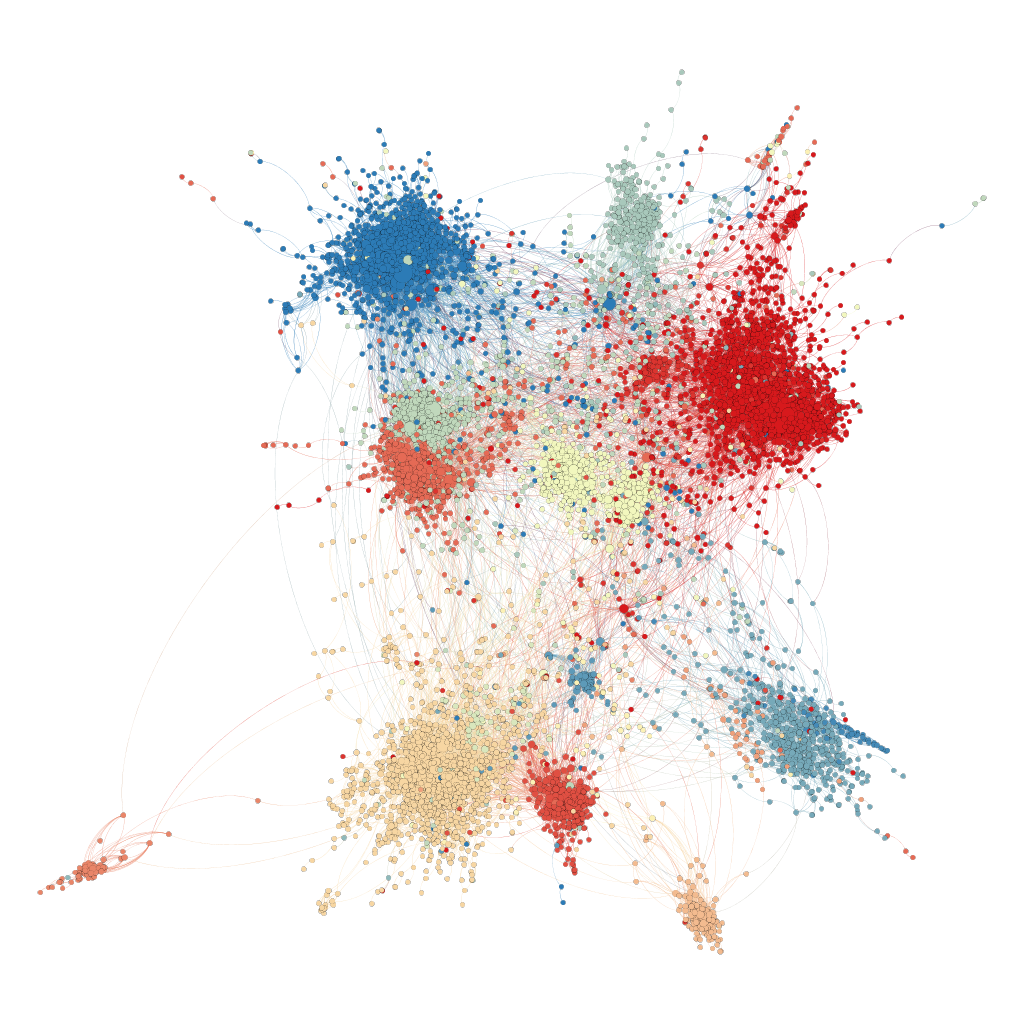
\includegraphics[width=1.097\textwidth]{img/resultados/grado-targets.png}
    \caption{Topología de la red. El color indica el país de cada usuario.}
\end{figure}

\begin{figure}[t]
    \centering
    \resizebox{0.78\columnwidth}{!}{%
    \begin{tabular}{| l | r |} 
        \hline
        \textbf{Medida} & \textbf{Valor} \\
        \Xhline{2\arrayrulewidth}
        Número de nodos \textbf{N} & 7,624 \\
        \hline
        Número de enlaces \textbf{L}	& 27,806 \\
        \hline
        Número máximo de enlaces \textbf{$L_{max}$} & 58117752 \\
        \hline
        Densidad del grafo \textbf{$L/L_{max}$} & 0.001 \\
        \Xhline{2\arrayrulewidth}
        Grado medio \textbf{<k>} & 7.294 \\
        \hline
        Diámetro \textbf{$d_{max}$} & 15 \\
        \hline
        Distancia media \textbf{d} & 5.232237269 \\
        \hline
        Coeficiente medio de clustering \textbf{<C>} & 0.285 \\
        \Xhline{2\arrayrulewidth}
        Número de componentes conexas & 1 \\
        \hline
        Número de nodos componente gigante (y \%) & 7,624 (100) \\
        \hline
        Número de aristas componente gigante (y \%) & 27,806 (100) \\
        \hline
    \end{tabular}
    }
    \caption{Medidas globales de la red.}
\end{figure}

    % ==============================================================================

    \setlength{\parskip}{1em}
    \newpage
    % \nocite{*}
    % \bibliography{bibliografia}
  	% \bibliographystyle{plain}
\end{document}